\section{Heater management}
This characteristic controls the heaters, so you can change the value of the heaters through the Gateway and you can modified the degrees of the thermometer through the Simulator.

To switch on/off and change the value of all heaters, follow the next steps:
\begin{enumerate}
\item Go to the global tab for the heaters in the Gateway window.
\begin{center}
	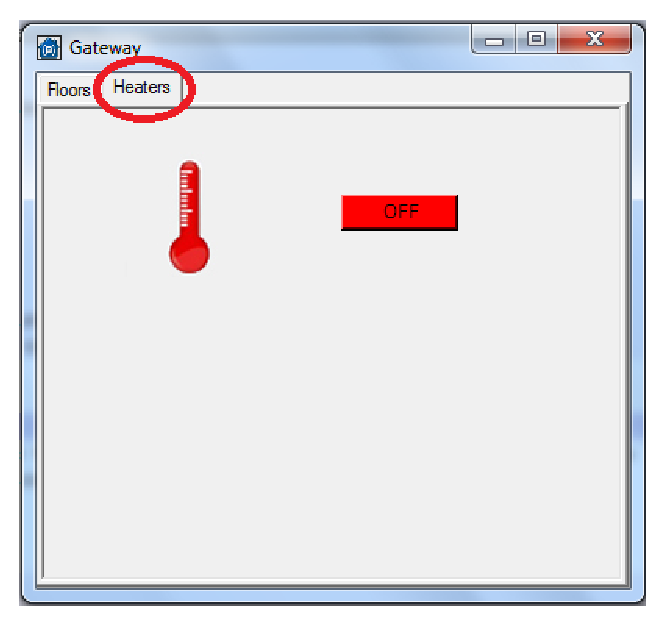
\includegraphics[width=.68\linewidth]{images/globalHeater.eps}
	\\
\vspace{1cm}
\end{center}
\item To switch on, click on the red button. Now, you can see in the Simulator window how the status of all heaters has changed.
\begin{center}
	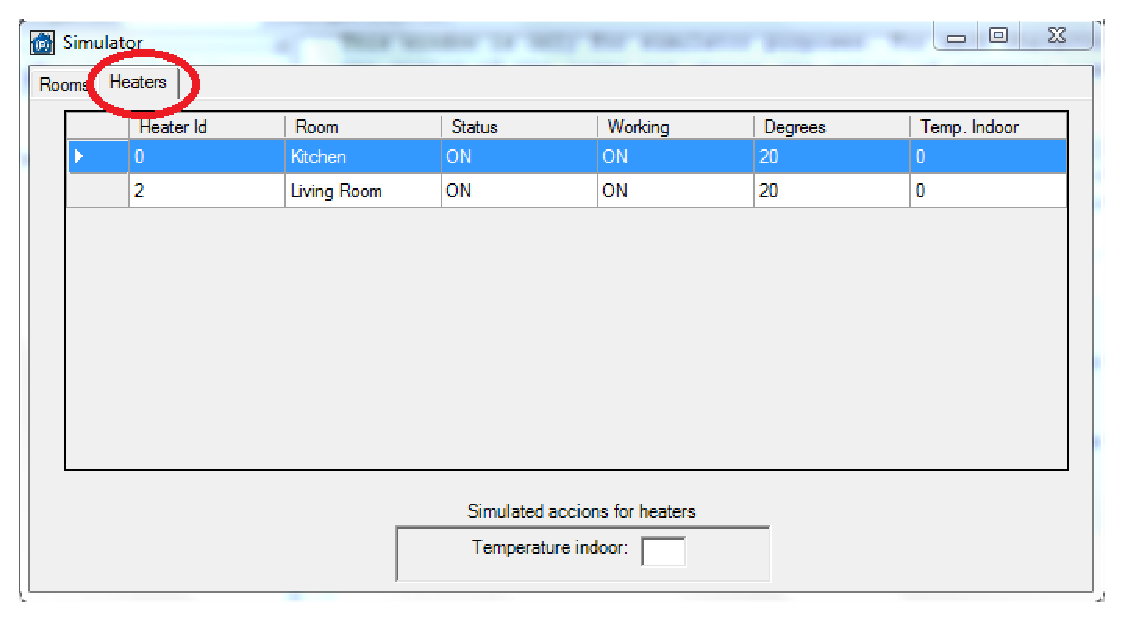
\includegraphics[width=.75\linewidth]{images/simulatorHeater.eps}
	\\
\vspace{1cm}
\end{center}
\item To change the temperature of the heaters, use the slide bar or the text box (press \emph{enter} key to confirm) to introduce a value between 0 to 40.
\begin{center}
	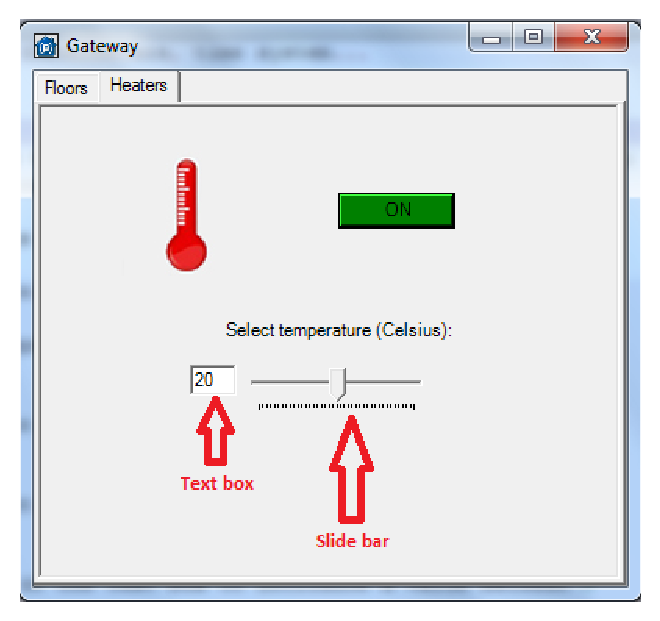
\includegraphics[width=.68\linewidth]{images/changeTemperatureHeater.eps}
	\\
\vspace{1cm}
\end{center}

\end{enumerate}
If you want to switch on/off or change the value of a specific heater, select the room where is the heater, click on the heater tab and follow the same steps to modified all heaters but in the current tab:
\begin{center}
	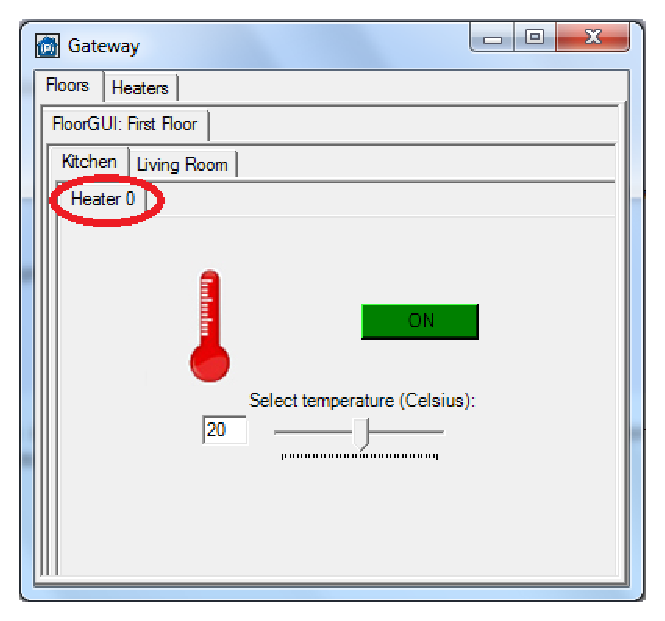
\includegraphics[width=.68\linewidth]{images/specificHeater.eps}
	\\
\vspace{1cm}
\end{center}

To change the value of a thermometer:
\begin{enumerate}
\item Go to Simulator window and select the heater tab.
\item Select a heater to change a specific thermometer. In the text box with the label \emph{Temperature indoor} introduce a value and press \emph{enter} key.
\begin{center}
	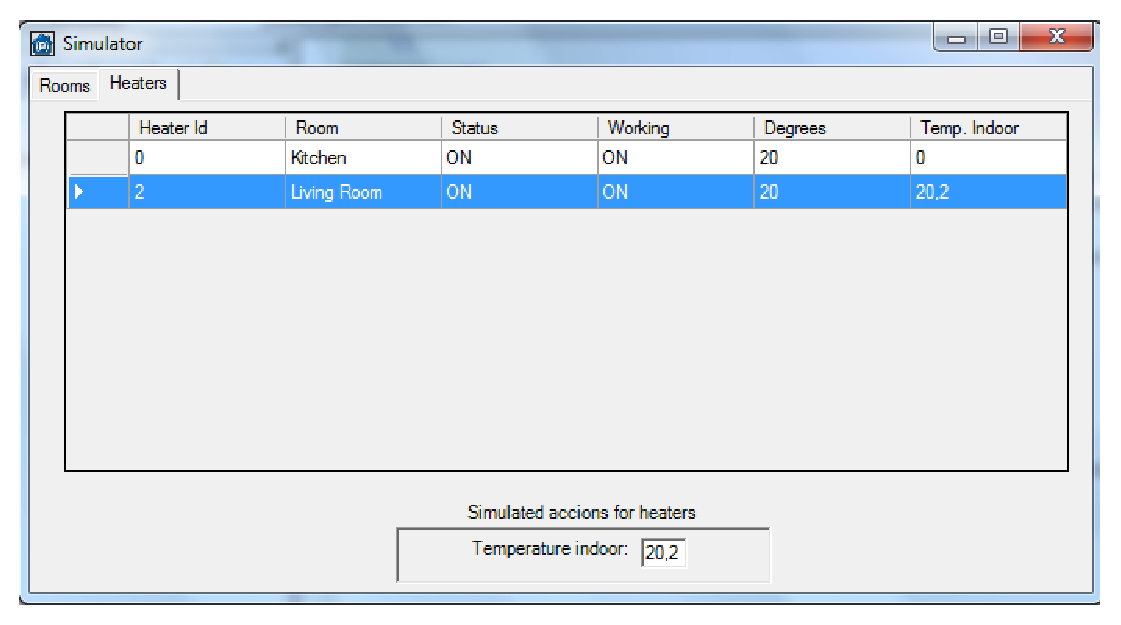
\includegraphics[width=.68\linewidth]{images/thermometerHeater.eps}
	\\
\vspace{1cm}
\end{center}
\end{enumerate}
If the temperature of a thermometer and its heater are equal, the heater will be \emph{OFF} in the \emph{Working} cell in the Simulator window, because of this, the heater won't waste energy. 